% !TeX encoding = UTF-8
% !TeX spellcheck = fr_FR


\chapter{Cahier des charges}
\label{s:cdc}

Ce chapitre explique la procédure utilisée dans le but d'établir le cahier des charges.
Il expose les barèmes des différents objectifs.
De plus, le cahier des charges est synthétisé dans le tableau \ref{t:cdc_tab} et dans la maison de la qualité à la figure \ref{t:cdc_mdlq}.

% !TeX encoding = UTF-8
% !TeX spellcheck = fr_FR


\section{Automatisation}
\label{s:cdc_autonm}

Cette partie est essentielle à la réalisation de notre projet. \cite{parker1991mise}
En effet, l’automatisation lui permettra d’être autonome, fiable et précis lors de la prise de données.
Ainsi cette partie a une pondération de 20~\%.
% !TeX encoding = UTF-8
% !TeX spellcheck = fr_FR


\section{Communication}
\label{s:cdc_comm}

Deux barèmes constitueront l’évaluation de ce critère.
Premièrement, le système doit être facilement joignable et utilisable sans nécessiter une formation.

% !TeX encoding = UTF-8
% !TeX spellcheck = fr_FR


\subsection{Accès à distance}
\label{s:cdc_com_accadist}

Dans le but de rendre le système autonome et simplifier l’utilisation de celui-ci, une communication à distance doit être configurée.
Cette caractéristique est cruciale étant donné de la position du capteur, qui n’est pas facilement accessible, car il est placé à une certaine profondeur dans l’eau.
C’est pourquoi une pondération de 10~\% lui est associée. Deux éléments principaux constitueront l’évaluation de ce critère.
Premièrement, le système doit admettre une communication rapide à distance en tout temps.
Selon l’atteinte de ce critère, une valeur entre 0 et 1 leur sera transmise selon la réussite ou l’échec du critère.
La valeur est déterminé par la vitesse de la connexion selon cette formule où $x$ est la vitesse de connexion en $ko/s$:
\begin{equation} \label{eq:4.1.1}
	\ln \left( \frac{x-384}{6816} \right) +1,\qquad x \in [384,\,7200]
\end{equation}
% !TeX encoding = UTF-8
% !TeX spellcheck = fr_FR


\subsection{Facilité d’utilisation}
\label{s:cdc_com_faciutil}

Afin de rendre l’utilisation du système plus efficace et plus accessible, une interface facilement accessible doit être configurée pour assurer la communication à distance.
Un site web pourra assurer une facilité de connexion avec le système pour que n’importe quel opérateur du MFA puisse utiliser le système sans problèmes.
Ce critère aura une pondération de 5~\%.
Une interface simple et facilement utilisable obtiendra une note de 1, une interface complexe et qui provoque la confusion obtiendra la note de 0,5 et l’absence d’interface donnera la note de 0.
% !TeX encoding = UTF-8
% !TeX spellcheck = fr_FR


\section{Coûts et échéances}
\label{s:cdc_coutsech}

% !TeX encoding = UTF-8
% !TeX spellcheck = fr_FR


\subsection{Coût du projet}
\label{s:cdc_cee_coutproj}

Ce critère est subdivisé en deux sous-catégories soit les coûts matériels et les coûts de main-d’œuvre.
La partie matérielle englobe l’ensemble des pièces et des produits qui seront utilisés pour mettre au point le capteur ainsi que la plateforme automatisée.
Le MFA a mis à notre disposition une somme maximale de 10 000~\$ pour rassembler les pièces nécessaires à la construction du produit.
Enfin, pour la partie main-d’œuvre, qui représente principalement le salaire des employés travaillant sur le projet, un total de 40 000~\$ pourra être utilisé au maximum.
Le barème est présenté au tableau \ref{tab:cdc_cee_coutproj}.

\begin{table}[H]
	\renewcommand\arraystretch{1.5}
	\centering
	\begin{tabular}{|l|c|c|}
		\hline
		& Pondération & Coût (\$)         \\ \hline
		\multirow{5}{*}{Coûts matériels}       & 0           & $[10000,\,\infty[$  \\ \cline{2-3}
		& 1.25 & $[7500,\,10000[$ \\ \cline{2-3}
		& 2.5 & $[5000,\,7500[$ \\ \cline{2-3}
		& 3.75 & $[2500,\,5000[$ \\ \cline{2-3}
		& 5 & $[0,2500[$ \\ \hline
		\multirow{5}{*}{Coûts de main-d’œuvre} & 0           & $[40000,\,\infty[$  \\ \cline{2-3}
		& 1.25 & $[30000,\,40000[$ \\ \cline{2-3}
		& 2.5 & $[20000,\,30000[$ \\ \cline{2-3}
		& 3.75 & $[10000,\,20000[$ \\ \cline{2-3}
		& 5 & $[0,10000[$ \\ \hline
	\end{tabular}
	\caption{Barème pour le coût du projet}
	\label{tab:cdc_cee_coutproj}
\end{table}
% !TeX encoding = UTF-8
% !TeX spellcheck = fr_FR


\subsection{Respect de l’échéance}
\label{s:cdc_cee_rspech}

La firme d’ingénieurs Sultan n’a pas reçu de date de remise du prototype précise.
Par contre, dans l’optique de montrer le professionnalisme de notre firme, le produit final sera livré au client dans les plus brefs délais, sans pour autant compromettre la qualité du projet.
Pour permettre une évaluation fluide de ce critère, la date du 18 avril 2019 représente l’objectif pour la remise du produit.
Le barème est calculé selon la formule \ref{eq:cdc_cee_rspech}, où $d$ est la date de remise par rapport au 18 avril 2019.

\begin{equation}
	\label{eq:cdc_cee_rspech}
	\left\{\begin{matrix}
		5, & d\le0\\ 
		-d+5, & d>0
	\end{matrix}\right.
\end{equation}
% !TeX encoding = UTF-8
% !TeX spellcheck = fr_FR


\section{Prise de données}
\label{s:cdc_prisdonn}

% !TeX encoding = UTF-8
% !TeX spellcheck = fr_FR


\subsection{Contrainte physique}
\label{s:cdc_pdd_cntphy}

Le client n’a pas indiqué de proportions claires à respecter pour la taille de notre système, celui-ci devra tout de même être le plus compact possible tout en assurant qu’une analyse sur un volume d’au moins un mètre cube d’eau soit possible.
Le système doit tolérer des températures entre 4~°C et 25~°C.
Afin d’éviter les problèmes de surchauffe, le produit final doit aussi compter un système de refroidissement automatique afin que la température intérieure soit au plus bas 10~°C en dessous de la température de l’eau et au plus haut cinq~°C au-dessus.
Le client demande aussi que le système soit assez résistant pour fonctionner à 15,25~m sous l’eau.
De plus, la limite de la masse de la partie submergée est fixée à 5 kilogrammes.
Un choix judicieux de matériaux légers, mais robustes est donc de mise.
Nous pondérons ce critère à 5~\%. Pour s’assurer de bien respecter ce critère, un tableau est fourni:

\begin{table}[htp]
	\caption{Barème de contraintes physiques}
	\label{tab:cdc_pdd_cntphy}
	\centering
	\begin{tabular}{|l|c|c|c|}
		\hline
		\multirow{2}{*}{\textbf{Partie évaluée}} & \multicolumn{3}{c|}{\textbf{Condition pour avoir la note de}} \\\cline{2-4}
		 & 0,2 & 0,15 & 0 \\\hline
		Volume analysé $V$ (m\textsuperscript{3}) & $V \ge 1$ & $V=1$ & $V<1$  \\\hline
		Température supportée $T$ (°C) & $4 \le T \le 25$  & non attribuée & 0 \\\hline
		Température par rapport à l'eau $\Delta T$ (°C) & $-10 \le \Delta T \le 5$ & non attribuée & 0 \\\hline
		Profondeur maximale $p$ (m) & $p \ge 15,25$ & $p=15,25$ & $p<15,25$    \\\hline
		Masse submergée $m$ (kg) & $m \ge 5$ & & $m < 5$  \\\hline
	\end{tabular}
\end{table}
% !TeX encoding = UTF-8
% !TeX spellcheck = fr_FR


\subsection{Capteur}
\label{s:cdc_pdd_capt}

Le client désire pouvoir récolter des données sur des spécimens d’au moins six centimètres.
Ainsi, il faut que la distance à laquelle la photo est prise résulte en une image d’au moins 16 pixels sur le capteur, ceux-ci étant le nombre maximal de pixels afin de pouvoir identifier quelque chose sur une photo.
Pour se faire, il faut que notre capteur produise une lumière suffisante à des distances maximales et minimales du volume d’analyse.
Il faut donc tenir compte de la relation inverse de la luminosité en fonction de la distance de la source.
Ce critère est important, car c’est celui qui assure la prise de photo qui est au cœur du projet. Ainsi on pondère ce critère à 5~\%.
Pour s’assurer du respect maximum de ce critère, la valeur de celui-ci est divisée en trois sous critères valant chacun 0,3 point, puis une fois que les valeurs seront additionnées, cela donnera un résultat sur 1.
% !TeX encoding = UTF-8
% !TeX spellcheck = fr_FR


\section{Sécurité}
\label{s:cdc_secu}

% !TeX encoding = UTF-8
% !TeX spellcheck = fr_FR


\subsection{Alarmes}
\label{s:cdc_sec_alar}

Selon la demande du client, le système sera composé d’un dispositif d’alarmes qui signalera l’opérateur dans le cas d’un problème.
Dans le cas d’un malfonctionnement ou d’un bris, une alarme sera levée à l’opérateur du MFA afin d’assurer une réparation rapide pour minimiser la période réfractaire.
Comme le système se trouve dans un milieu éloigné, il est important de savoir si le système fonctionne ou non.
C’est pourquoi une pondération de 5~\% sera affectée à ce critère.
Comme note, 1 sera attribué si les alarmes sont fonctionnelles et 0 si les alarmes sont absentes.
% !TeX encoding = UTF-8
% !TeX spellcheck = fr_FR


\subsection{Protection de l’accès à distance}
\label{s:cdc_sec_protaccdist}

Selon la demande du client, la transmission des informations et des alarmes doit être faite sur une connexion sécurisée avec le système en parallèle avec la communication à distance.
L’interception et le détournement des données pourraient avoir un impact nocif pour le fonctionnement du système (alarmes) et du logiciel de traitement (base de données).
Comme le système peut être dans un endroit éloigné comme dans un lac et difficilement détectable, il sera difficile pour un intrus de détecter le système et la connexion.
C’est pourquoi sa pondération sera de 4~\%.
L'équation \ref{eq:cdc_sec_protaccdist} calcule le barème, où $b$ est la longueur de la clé de chiffrement en bits.

\begin{equation}\label{eq:cdc_sec_protaccdist}
	\left(\frac{b-128}{960}\right)^2
\end{equation}
% !TeX encoding = UTF-8
% !TeX spellcheck = fr_FR


\subsection{Protection des données du client}
\label{s:cdc_sec_protdonnclnt}

Selon la demande du client, la base de données où seront enregistrées les données doit être sécurisée et confidentielle.
Il est important d’assurer ce critère, car toutes les images prises pour la détection doivent être stockées pendant une période d’au moins 2 ans selon la demande du client.
De plus, un intrus qui réussit à récupérer le système ne doit pas pouvoir accéder aux données, car la confidentialité de celles-ci sera compromise.
C’est pourquoi une pondération de 4~\% sera affectée à ce critère.
Comme note, 1 sera attribué si la sécurité de la base de données et la sécurité de l’accès physique au système est assurée, 0,5 si un seul de ces deux critères est assuré et 0 si elle n’est pas sécurisée.
% !TeX encoding = UTF-8
% !TeX spellcheck = fr_FR


\subsection{Protection de l’environnement}
\label{s:cdc_sec_protenv}

Comme la tâche qu’accomplit le système nécessite un écosystème aquatique en santé, il est important que celui-ci n’affecte pas l’environnement qu’il tente d’évaluer.
En cas de bris, le système doit être hermétique pour éviter les fuites dans le milieu.
Afin de protéger le système et les poissons qu’il évalue, il faudra accorder une attention particulière pour éviter que le système court-circuite avec l’eau et endommage l’écosystème.
C’est pourquoi une pondération de 2~\% sera affectée à ce critère.
Comme note, 1 sera attribué s’il n’y a aucun impact sur l’environnement et 0 s’il a un impact nocif sur l’écosystème.
% !TeX encoding = UTF-8
% !TeX spellcheck = fr_FR


\section{Stockage de données}
\label{s:cdc_stockage}

Le stockage se voit attribué 10~\% de la pondération totale.

% !TeX encoding = UTF-8
% !TeX spellcheck = fr_FR


\subsection{Durée de conservation des données}
\label{s:cdc_stock_duree}

Le client exige que le système soit en mesure d’archiver les fichiers pour une période à court et long terme. La période la plus courte est de 14 jours alors que la plus longue est plutôt de 2 ans. L’évaluation de ce critère se fait en deux volets, chaque volet a une valeur de 1,5~\%, donc si les deux critères sont parfaitement réussis, un score de 1 est attribué. 

\begin{table}[htp]
	\caption{Barème pour la conservation des données}
	\label{t:cdc_stock_duree}
	\centering
	\begin{tabular}{|l|l|}
		\hline
		\textbf{Conservation} & \textbf{Pondération}                                                                              \\ \hline \hline
		Données locales       & \begin{tabular}[c]{@{}l@{}}\textless 14 jour : 0\%\\ $\geq$ 14 jours: 1,5\%\end{tabular} \\ \hline
		Données dans le nuage & \begin{tabular}[c]{@{}l@{}}\textless 2 ans : 0\%\\ $\geq$ 2ans: 1,5\%\end{tabular}       \\ \hline
	\end{tabular}
\end{table}

La pondération pour ce critère est de 3~\%, car les données doivent être conservées sur deux périodes distinctes.
% !TeX encoding = UTF-8
% !TeX spellcheck = fr_FR


\subsection{Stockage local}
\label{s:cdc_stock_local}

La portion du système qui sera submergée au fond du cours d’eau doit posséder une mémoire locale où les images prises par le capteur seront emmagasinées jusqu’à ce que ces fichiers ne soient définitivement transférés dans la banque à long terme (voir le critère suivant). Puisque la quantité à stocker est minime, il est important que la mémoire ne soit pas énergivore et que l’espace qu’elle occupe soit limitée. Considérant l'image originale et des vignettes de 100 par 100 pixels, la quantité de photos prises par le capteur à quelques centaines au courant de la période de 14 jours, une simple carte SD de 64 Go offre un coussin confortable. L’évaluation de ce critère se fait à l’aide de l'équation \ref{eq:cdc_stock_local} où x représente la mémoire local en Go. 

\begin{equation} \label{eq:cdc_stock_local}
	\frac{x}{32}, \qquad x \in [0,\,32]
\end{equation}

Une pondération de 3~\% est octroyée à ce critère puisque de nombreuses solutions simples, accessibles et peu coûteuses existent. 

% !TeX encoding = UTF-8
% !TeX spellcheck = fr_FR


\subsection{Stockage dans le nuage}
\label{s:cdc_stock_nuage}

L’ensemble des images capturées par la caméra seront par la suite archivées dans un nuage où ces images seront conservées pour une durée de 2 ans avant d’être ensuite supprimées. Considérant la petite taille des photos, un nuage d’une centaine de GO est amplement suffisant et il est pratiquement impossible de saturer le nuage en raison de la taille des fichiers sauvegardés. Le barème pour ce critère fonctionne de la même manière que pour le stockage local, sauf que la mémoire est de 1 To. On obtient ainsi l’équation \ref{eq:cdc_stock_nuage}. Donc, on remarque que un pointage de 1 est attribué pour un stockage de 1 To dans le nuage et le pointage de 0 pour un stockage nul.

\begin{equation} \label{eq:cdc_stock_nuage}
x, \qquad x \in [0,\,1]
\end{equation}


La pondération pour ce critère est de 4~\%, car une quantité considérablement plus grande de photos doivent être stockées comparativement à la mémoire locale.

% !TeX encoding = UTF-8
% !TeX spellcheck = fr_FR


\newpage

\begin{table}[htp]
	\caption{Tableau du cahier des charges}
	\label{t:cdc_tab}
	\centering
	\begin{tabular}{|l|c|c|c|c|}
		\hline\hline
		\textbf{\textit{Critères d’évaluation}} & \textbf{\textit{Pond. (\%)}} & \textbf{\textit{Barème}} & \textbf{\textit{Min}} & \textbf{\textit{Max}} \\
		\hline
		\hline
		\ref{s:cdc_autonm} \textbf{Automatisation} & \textbf{20} & & & \\
		\ref{s:cdc_aut_autnmi} Autonomie & 7 & Équation \ref{eq:cdc_aut_autnmi} & & \\
		\ref{s:cdc_aut_basedonn} Base de données & 3 & & & \\
		\ref{s:cdc_aut_config} Configurabilité & 7 & & 0 & 100 \\
		\ref{s:cdc_aut_fiabsys} Fiabilité du système & 3 & & & \\
		\hline
		\hline
		\ref{s:cdc_comm} \textbf{Communication} & \textbf{15} & & & \\
		\ref{s:cdc_com_accadist} Accès à distance & 10 & Équation \ref{eq:cdc_com_accadist} & & \\
		\ref{s:cdc_com_faciutil} Facilité d’utilisation & 5 & & & \\
		\hline
		\hline
		\ref{s:cdc_coutsech} \textbf{Coûts et échéances} & \textbf{15} & & & \\
		\ref{s:cdc_cee_coutproj} Coût du projet & 10 & Tableau \ref{tab:cdc_cee_coutproj} & & \\
		\ref{s:cdc_cee_rspech} Facilité d’utilisation & 5 & Tableau \ref{tab:cdc_cee_rspech} & & \\
		\hline
		\hline
		\ref{s:cdc_prisdonn} \textbf{Prise de données} & \textbf{10} & & & \\
		\ref{s:cdc_pdd_cntphy} Contrainte physique & 5 & Tableau \ref{tab:cdc_pdd_cntphy} & & \\
		\ref{s:cdc_pdd_capt} Capteur & 5 & & & \\
		\hline
		\hline
		\ref{s:cdc_secu} \textbf{Sécurité} & \textbf{15} & & & \\
		\ref{s:cdc_sec_alar} Alarmes & 5 & & & \\
		\ref{s:cdc_sec_protaccdist} Protection de l’accès à distance & 4 & & & \\
		\ref{s:cdc_sec_protdonnclnt} Protection des données du client & 4 & & & \\
		\ref{s:cdc_sec_protenv} Protection de l’environnement & 2 & & & \\
		\hline
		\hline
	\end{tabular}
\end{table}
% !TeX encoding = UTF-8
% !TeX spellcheck = fr_FR


\newpage

\begin{figure}[htp]
	\centering
	\caption{Maison de la qualité}
	\label{f:cdc_maison}
	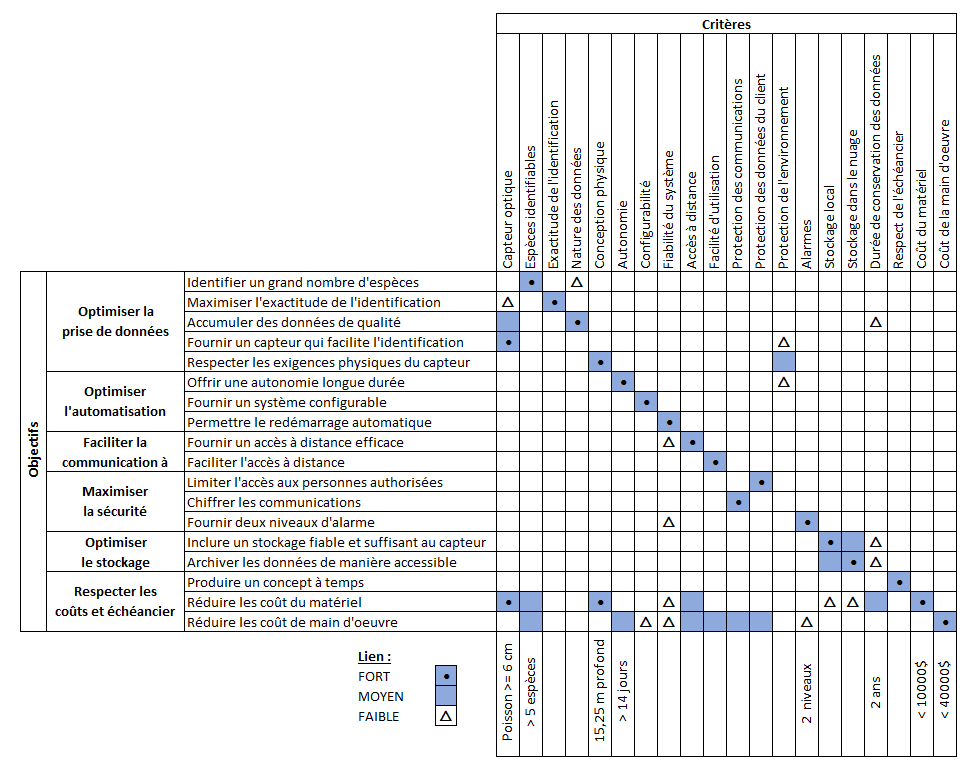
\includegraphics[width=\textwidth]{maison_qualite.png}
\end{figure}